\subsection{Coloring with 4 registers}

\begin{figure}[!htbp]
    \centering
    \caption{Determining live ranges and merged live ranges.}
    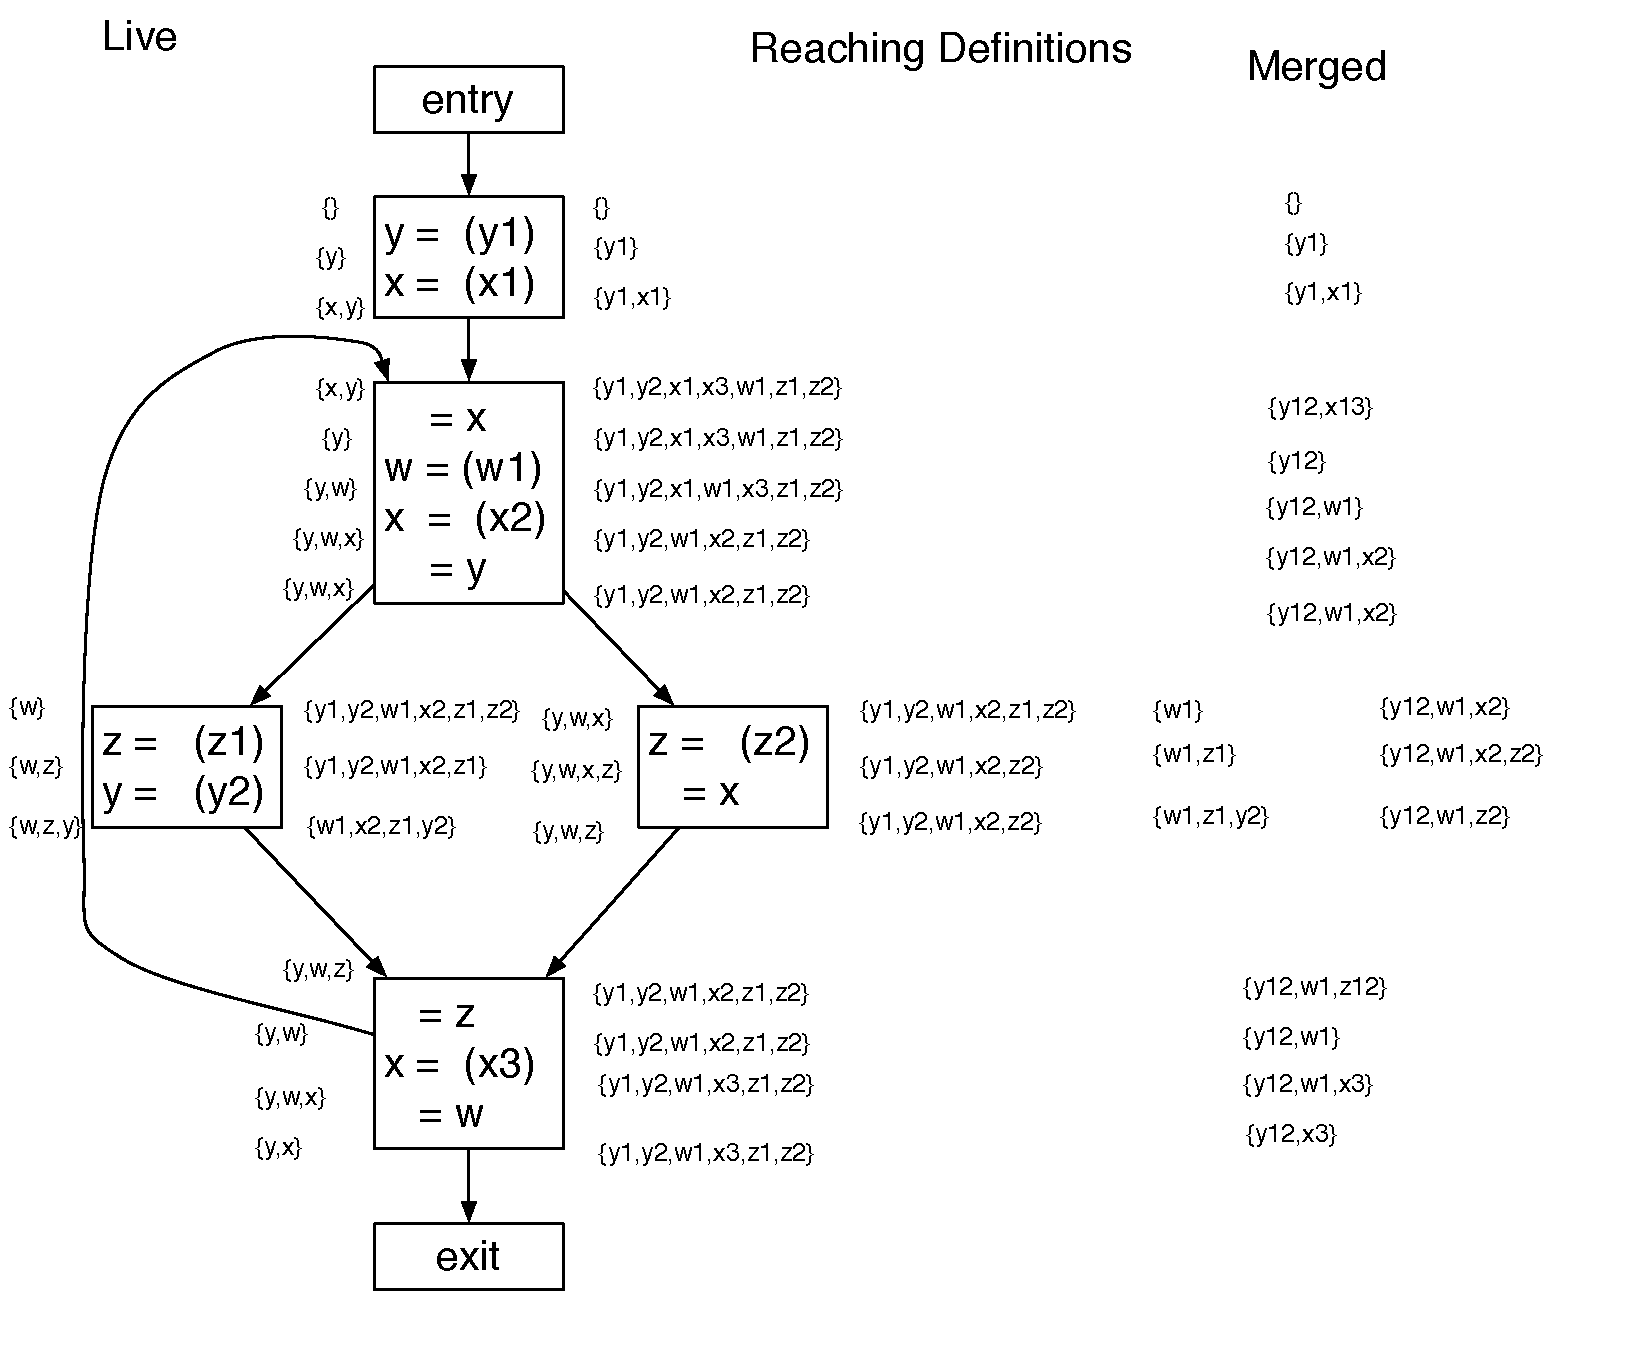
\includegraphics[scale=0.50]{register_allocation1.pdf}
    \label{fig:regalloc1}
\end{figure}

\clearpage

\begin{figure}[!htbp]
    \centering
    \caption{Building the interference graph.}
    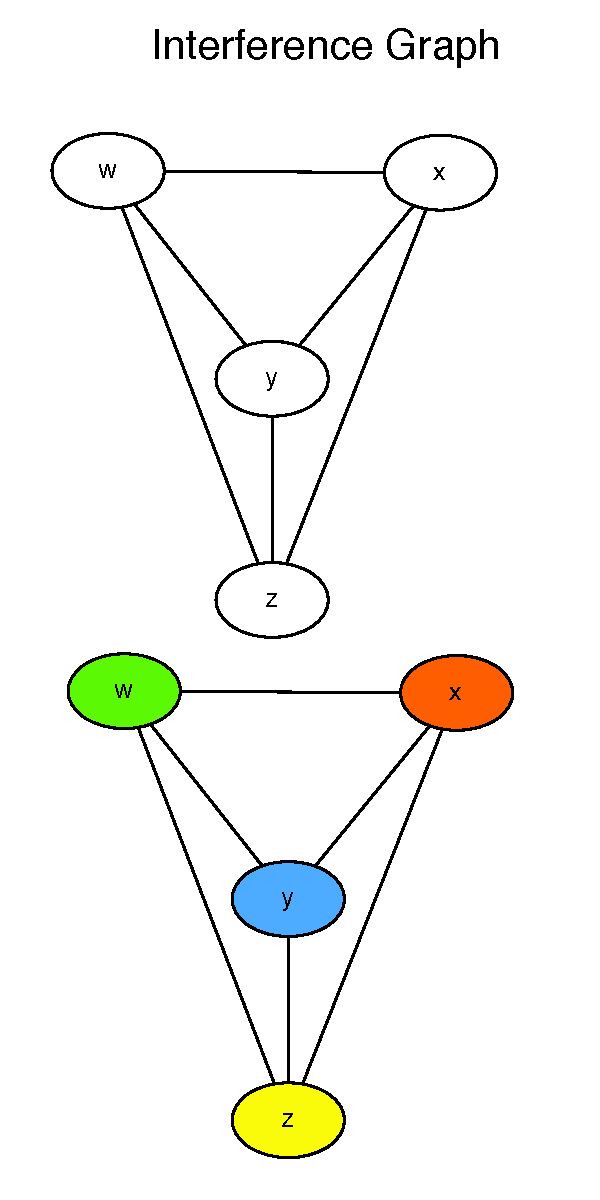
\includegraphics[scale=0.60]{register_allocation2.pdf}
    \label{fig:regalloc2}
\end{figure}

\clearpage

\begin{figure}[!htbp]
    \centering
    \caption{Rewriting the code.}
    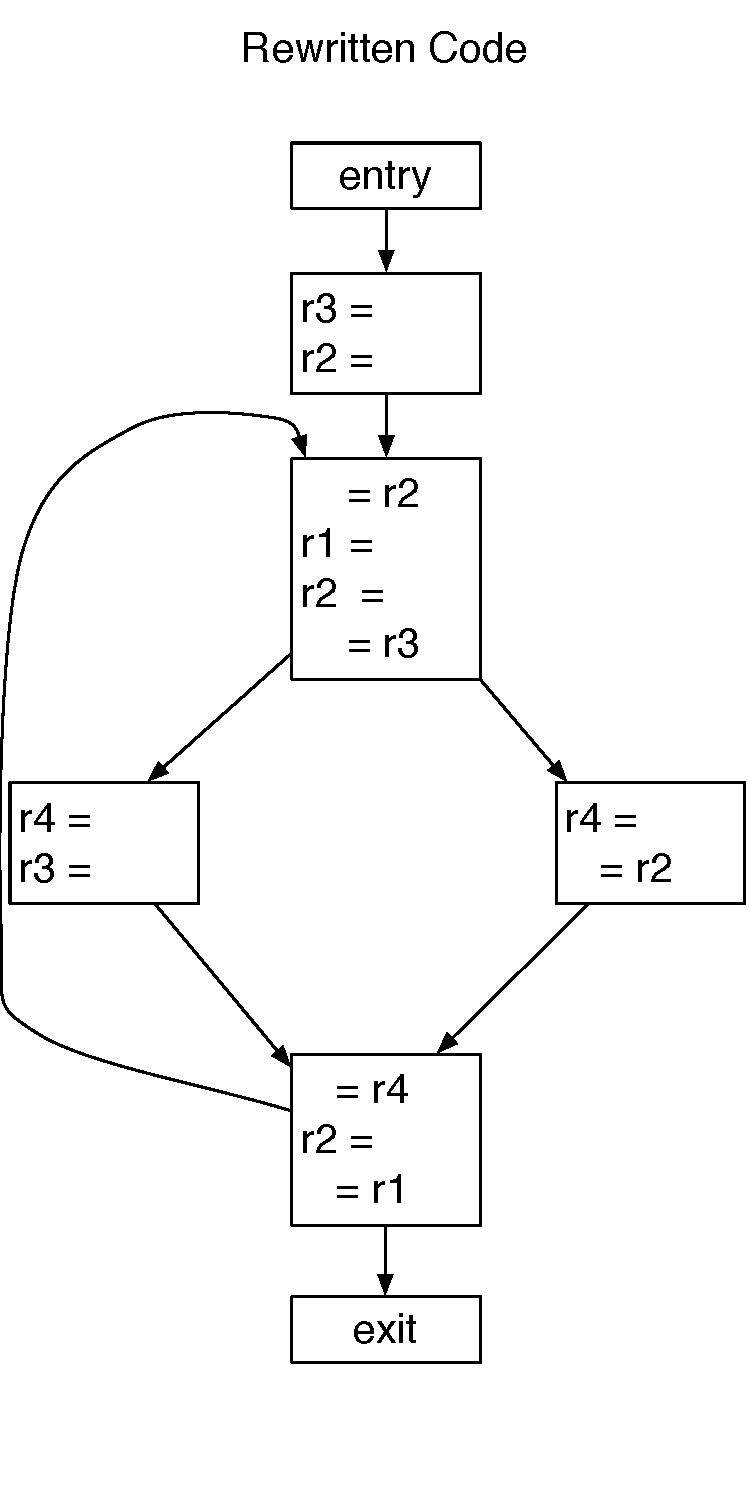
\includegraphics[scale=0.50]{register_allocation3.pdf}
    \label{fig:regalloc3}
\end{figure}

\subsection{Coloring with 3 registers}

No, it's not possible to color the graph using only 3 colors! We have to spill some register to memory.
We can use different approaches to split one register to memory. We will use a simple heuristic (from class),
where we compute the cost of spilling each variable, namely:

$\mathtt{cost} = [(\# \mathtt{defs} + \mathtt{uses}) * 10^{\mathtt{loop-nest-depth}}]/\mathtt{degree}$

We know that $\mathtt{loop-nest-depth} = 1$ for all variables.

\begin{center}
    \begin{tabular}{ | l | l | l | l | l | l |}
    \hline
    Variable & Uses & Defs & Degree & Cost \\ \hline
    w & 1 & 1 & 3 & 6.6 \\ \hline
    x & 2 & 3 & 3 & 16.6 \\ \hline
    y & 1 & 2 & 3 & 10.0 \\ \hline
    z & 1 & 2 & 3 & 10.0 \\ \hline
    \hline
    \end{tabular}
\end{center}

The variable with the least cost is $w$, therefore we will spill $w$ to memory.